% Name: Feedback loop with disturbance and noise
% Description: A feedback loop with a disturbance added to the plant output and sensor noise added to the measurement.
% Tags: feedback, disturbance, noise, control systems

\usetikzlibrary{arrows.meta}

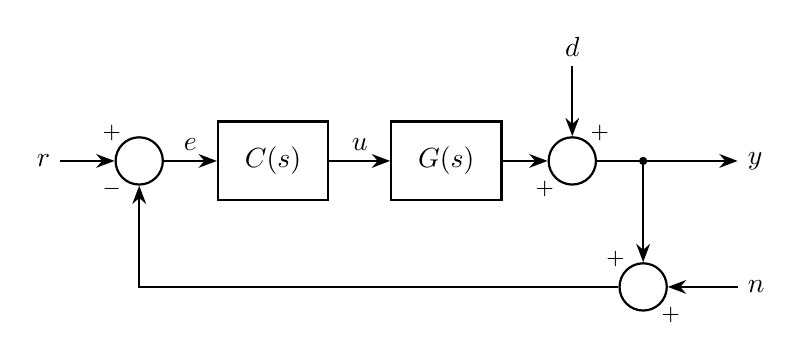
\begin{tikzpicture}[
  block/.style={draw, thick, minimum height=10mm, minimum width=14mm},
  sum/.style={draw, thick, circle, inner sep=0pt, minimum size=6mm},
  arrow/.style={-{Stealth}, thick},
  sign/.style={font=\footnotesize},
]
  \node[sum] (s1) at (1,0) {};
  \node[block] (C) at (2.7,0) {$C(s)$};
  \node[block] (G) at (4.9,0) {$G(s)$};
  \node[sum] (s2) at (6.5,0) {};
  \node[sum] (s3) at (7.4,-1.6) {};

  \draw[arrow] (0,0) node[left] {$r$} -- (s1);
  \draw[arrow] (s1) -- node[above] {$e$} (C);
  \draw[arrow] (C) -- node[above] {$u$} (G);
  \draw[arrow] (G) -- (s2);
  \draw[arrow] (s2) -- (8.6,0) node[right] {$y$};
  \draw[arrow] (6.5,1.2) node[above] {$d$} -- (s2);
  \draw[arrow] (7.4,0) -- (s3);
  \draw[arrow] (8.6,-1.6) node[right] {$n$} -- (s3);
  \draw[arrow] (s3) -| (s1);
  \fill (7.4,0) circle (1.5pt);

  \node[sign] at ([shift={(-3.5mm,3.5mm)}]s1) {$+$};
  \node[sign] at ([shift={(-3.5mm,-3.5mm)}]s1) {$-$};
  \node[sign] at ([shift={(3.5mm,3.5mm)}]s2) {$+$};
  \node[sign] at ([shift={(-3.5mm,-3.5mm)}]s2) {$+$};
  \node[sign] at ([shift={(-3.5mm,3.5mm)}]s3) {$+$};
  \node[sign] at ([shift={(3.5mm,-3.5mm)}]s3) {$+$};
\end{tikzpicture}
